%!TEX TS-program = pdflatex
%!TEX root = main.tex
%!TEX encoding = UTF-8 Unicode

\section{Tempi}
%Usando \emph{multi\_batch\_plot.Rmd}
I grafici che seguono sono stati generati usando R e \emph{ggplot}.
%I valori usati per H e K sono gli interi tra 1 e 10, fissato un numero di corridoi vengono generati tutti gli input 

\noindent
In \autoref{fig:second_plot} si vede come il tempo totale di risoluzione degli input dati.
Notare come in genere il modello Minizinc sia migliore del modello ASP.
I pallini indicano se il modello è andato in timeout.
L'andamento del grafico è dato dal modo in cui sono stati generati gli input, quindi dal loro ordinamento: durante la generazione venivano effettuati due cicli for annidati uno per il numero di corridoi ed uno per il numero di stanze.
Quindi, come ci si può aspettare, la complessità dell'istanza cresce al crescere combinato di K ed H.
\begin{figure}[ht]
  \centering
  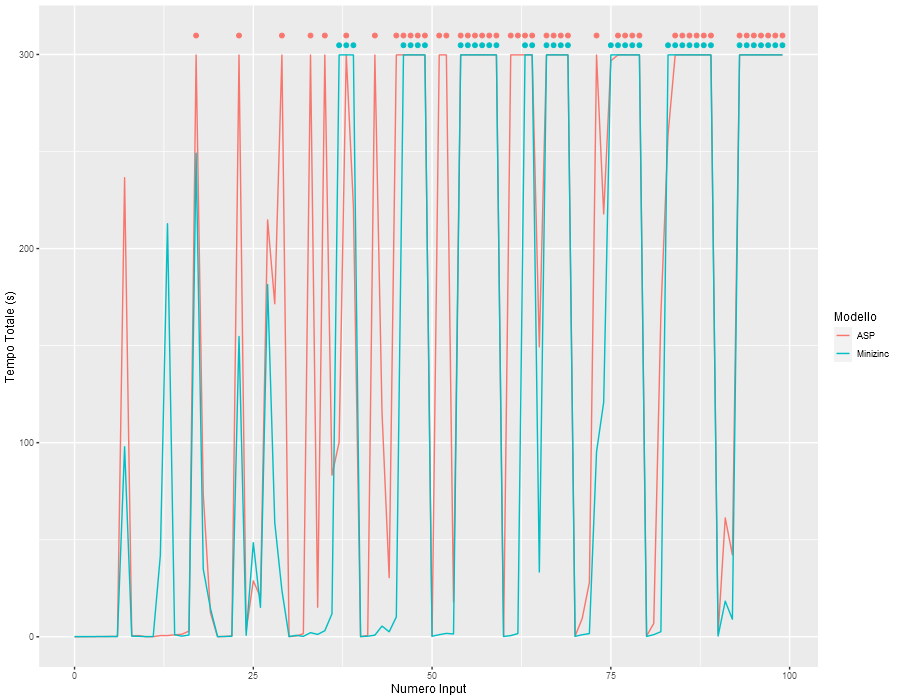
\includegraphics[width=\textwidth]{second_plot}
  \caption{Input in ordine di numerazione}
  \label{fig:second_plot}
\end{figure}

In \autoref{fig:first_plot} si vede il tempo di risoluzione.
\begin{figure}[ht]
  \centering
  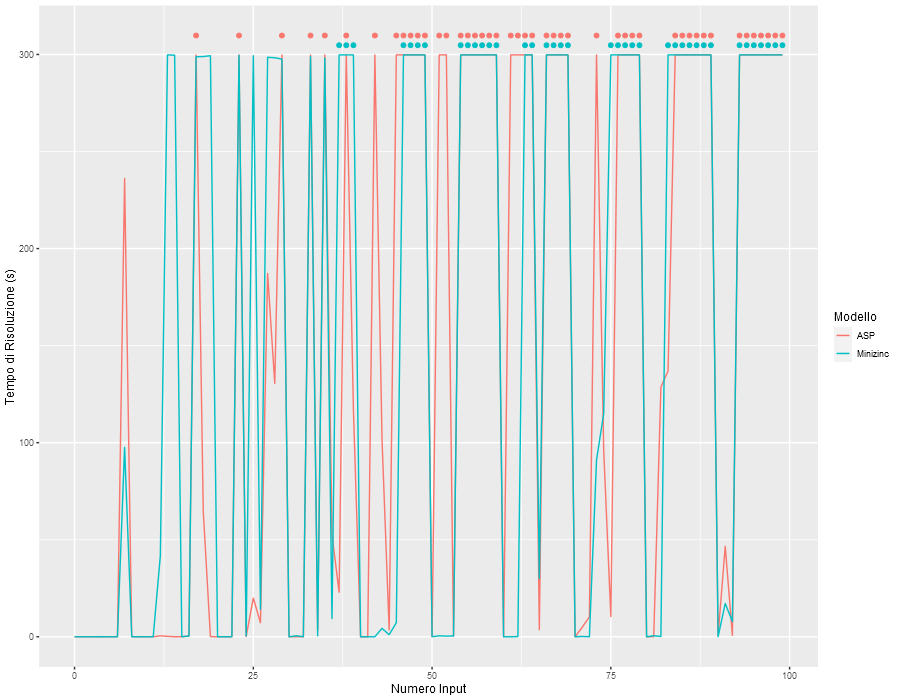
\includegraphics[width=\textwidth]{first_plot}
  \caption{Input in ordine di numerazione}
  \label{fig:first_plot}
\end{figure}
\cleardoublepage

Osservando soltanto le soluzioni per le quali non si è raggiunto il timeout ed ordinando secondo tempo totale di risoluzione del modello ASP si ottiene il grafico in \autoref{fig:no_timeout_times}.
\begin{figure}[ht]
  \centering
  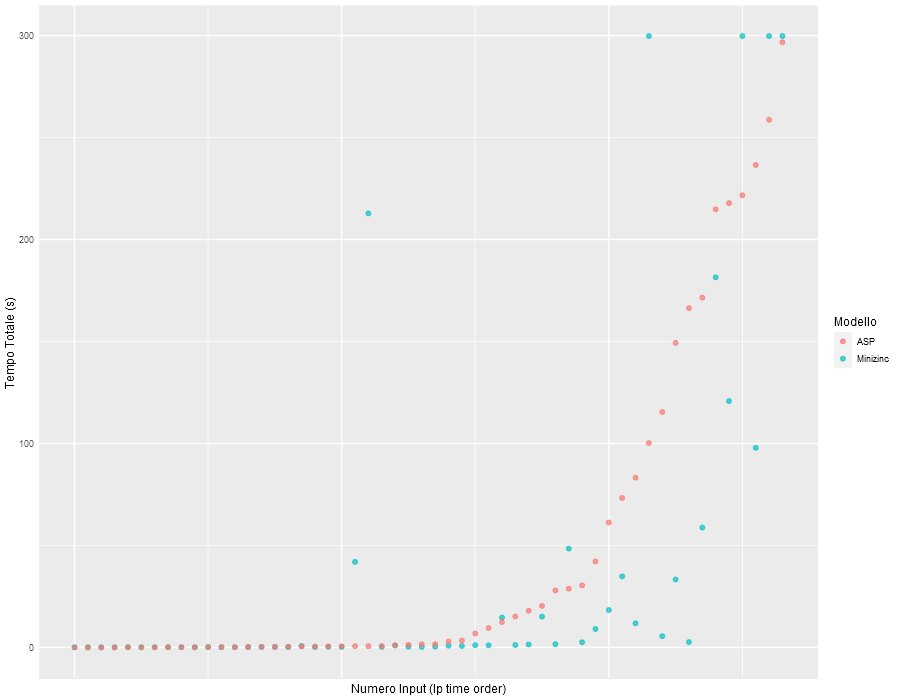
\includegraphics[width=.8\textwidth]{sorted_lp_time_no_timeout_times}
  \caption{Input in ordine crescente di tempo totale per il modello ASP}
  \label{fig:no_timeout_times}
\end{figure}
Notare come in più occasioni un modello performa molto bene mentre l'altro ha difficoltà.
Una delle cause di questo fenomeno è il modo in cui il modello Minizinc cerca le soluzioni, cioè iniziando a collocare gli ospiti in quarantena nelle stane più lontane e dei piani più alti.
Ciò non viene fatto nel modello ASP.
Le osservazioni appena fatte valgono anche per il tempo di risoluzione, come si vede in \autoref{fig:no_timeout_solvetimes}.
\begin{figure}[ht]
  \centering
  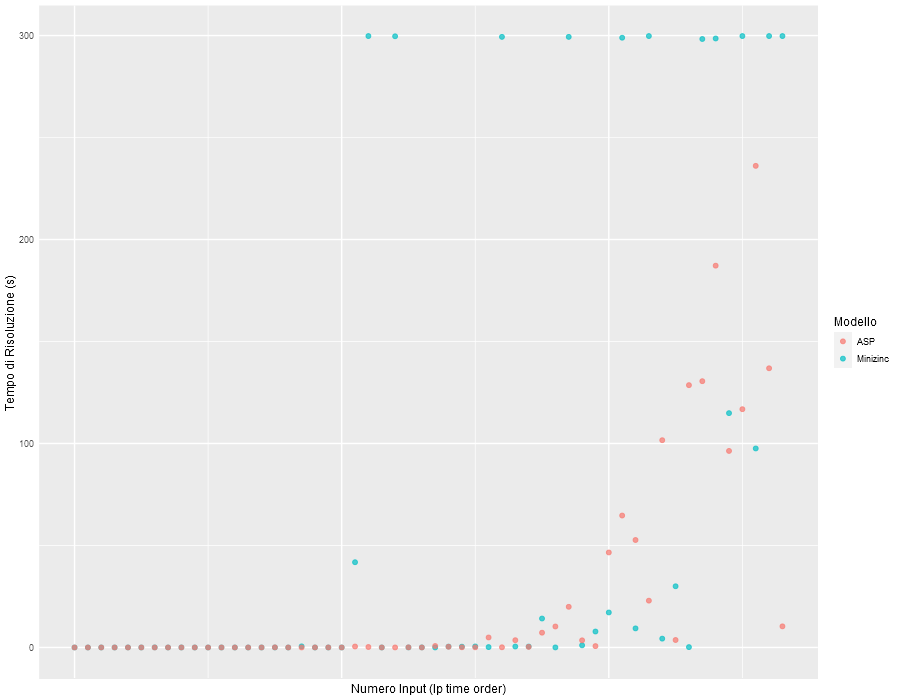
\includegraphics[width=.8\textwidth]{sorted_lp_time_no_timeout_solveTimes}
  \caption{Input in ordine crescente di tempo totale per il modello ASP}
  \label{fig:no_timeout_solvetimes}
\end{figure}
